\documentclass[12pt,fleqn]{article}\usepackage{../../common}
\begin{document}
Ders 2.3

Her hesapsal yöntemin doğruluğu ve stabilitesini bilmek isteriz. En basit
başlangıç değer problemi (initial value problem -IVP-) ile başlayalım,

$$
\frac{\partial u}{\partial t} =
c \frac{\partial u}{\partial x}
\mlabel{1}
$$

Buna tek yön dalga denklemi diyebiliriz, iki yönlü dalga denklemi için üstteki
formülde ikinci türevlerin olması gerekirdi, o tür denklemde dalgalar iki yöne
de giderdi. Üstteki tek yöne dalga gönderiyor, basit, temiz bir denklem, birinci
derece, hız bağlamında sabit katsayılı. Başlangıç değer problemi için başlangıç
değeri $u(x,0)$ ile verilmiş olsun, ve benim ilgilendiğim $u(x,t)$ çözümü.

Bu çözümü bulmak zor olmaz, mesela ilk aklıma gelen pür üsteller, $e^{ikx}$.  Bu
çözümün bir özelliği sabit katsayısı var, sınırı yok, o zaman çözüm $e^{ikx}$'in
bir katı olacak, bu demektir ki değişken ayırma tekniğini uygulayabilirim, ve $u
= G(x,t) e^{ikx}$ şeklinde bir çözüm bekleyebilirim. Nasıl değişkenler ayrıldı
görüyoruz, $G$ içinde $x$, $t$'den ayrıldı, ve frekans $k$ büyüme faktörü $G$'yi
tanımlıyor.

Çözümü bulmak için içinde $G$'yi içeren $u$ formülünü ana türevsel denklem (1)'e
sokarım, ve $t$'li çözümü elde ederim, çünkü $e^{ikx}$ iptal olacak. Formüle
sokayım,

$$
\frac{\ud G}{\ud t} e^{ikx} = ikc G e^{ikx}
$$

Ustelli kismi iptal ederim, o terimler hic sifir olmazlar nasilsa,

$$
\frac{\ud G}{\ud t} \cancel{e^{ikx}} = ikc G \cancel{e^{ikx}}
$$

Böylece $G$ için basit bir denkleme erişiyorum,

$$
\frac{\ud G}{\ud t} = ikc G 
$$

Sonuç sabit bir katsayıya dayaniyor, $ick$ katsayısına. Nihai denklemin bir
basit diferansiyel denklem olduğunu da farkediyoruz, o zaman çözüm yine
bir üstel, $G = e^{ikc t}$. Bu $G$'yi $u$ çözümü içine koyunca, 

$$
u = G(x,t) e^{ikx}
$$

$$
u = e^{ikc t} e^{ikx} = e^{ik(x + ct)} 
$$

Çözüm bu işte. Değişkenleri ayırdık, büyüme faktörüne baktık, bir üsteli
denedik, farklılık (difference) metotları için de aynısını yapacağız. Von
Neumann'ın dahice fikri buydu, üstelleri takip et. Her frekansa bak, ve
$e^{ikx}$'in katlarına neler olduğuna bak. 

İlginç bir şey, tüm frekanslar $x+ct$ kombinasyonunu ortaya
çıkarıyor. Fourier'in de söylediği bu değil miydi? $e^{ikx}$ kombinasyonlarını
alın, onların çözümü $e^{ik(x + ct)}$'lerin kombinasyonu olacak. Yani
$x$'ler $x+ct$ oluyor bir bakıma. O zaman çözüm

$$
u(x,t) = u(x+ct, 0)
$$

Bu her $u$ için.

Bu çözümün ne olduğunu sezgisel olarak rahatça anlayabiliriz tabii, bu
tek yöne giden bir dalga. Cebirde açıkca görülüyor. $x,t$ düzleminde
bir resim çizince daha da iyi görülebilir. Bu resmi anlamak önemli
çünkü farklılık yöntemi ile üstteki denklemi çözmeye uğraşıyoruz.

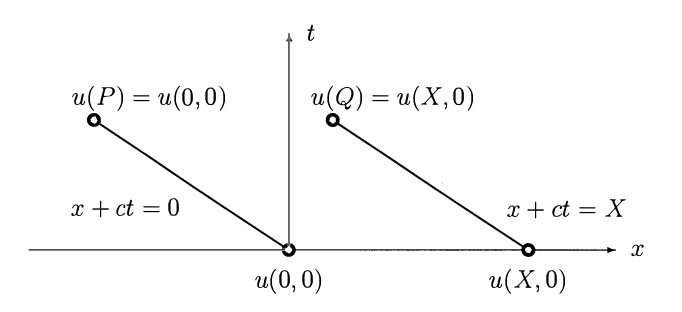
\includegraphics[width=20em]{compscieng_2_03_01.png}

Şimdi $u$'nun $(0,0)$ noktasındaki değerini düşünelim. Zaman geçtikten sonra
$x+ct$ çizgisindeki herhangi bir yerde, $P$'de olduğumuzu düşünelim, orada çözüm
hep aynı. Başlangıçtaki değer ne ise o çizgi (üstteki grafikte solda görülen)
üzerinde seyahat ediyor, $u$ değeri $(0,0)$'da ne $P$'de de o.

Üstte sağdaki çizgi aynı şekilde, orada da $X$ ile işaretli bir sabit değerde
başlayan değer çizgi üzerinde yukarı taşınacak, $Q$'da aynı $u$ değeri olacak.
[Dikkat, $x$ eksenindeki $X$ değeri $x+ct = X$ çizgisiyle temsil edilir
denmiyor, $x$ eksenindeki bir değer ile $.. =X$ şeklindeki bir çizginin
cebirsel bağlantısı yok, $ax+by+c=0$ denklemindeki sabitler grafiksel kesim
noktalarına tekabül etmezler].

Bu çizgilere karakteristik çizgiler (characteristic lines) ismi veriliyor.














[devam edecek]

\end{document}

